% Biên dịch: latexmk -xelatex Report.tex   (Overleaf: Compiler = XeLaTeX)
% Ảnh chụp terminal và logo trường nằm trong images/.
% BẢN NHÁP: các khối todobox và \tbd đánh dấu phần chưa hoàn thiện
% (Task 3.3, Task 3.4, make grade đầy đủ, time.txt). Xóa hết trước khi nộp.
\documentclass[10pt,a4paper]{article}
\usepackage[left=2cm,right=1.8cm,top=2.1cm,bottom=1.9cm,headheight=14pt,headsep=12pt,footskip=22pt]{geometry}
\usepackage{fontspec}
\setmainfont{texgyretermes}[Extension=.otf,UprightFont=*-regular,BoldFont=*-bold,
  ItalicFont=*-italic,BoldItalicFont=*-bolditalic]
\setmonofont{DejaVuSansMono}[Path=fonts/,Extension=.ttf,UprightFont=*,BoldFont=*-Bold,
  ItalicFont=*-Oblique,BoldItalicFont=*-BoldOblique,Scale=0.86]
\usepackage{polyglossia}
\setdefaultlanguage{vietnamese}
\usepackage[table]{xcolor}
\usepackage{graphicx,booktabs,tabularx,array,multirow,etoolbox,enumitem,titlesec,
  caption,float,fancyhdr,lastpage,listings,fancyvrb,tikz,multicol,needspace}
\usepackage[most]{tcolorbox}
\usetikzlibrary{arrows.meta,calc,positioning,patterns}
\usepackage{hyperref}

% ------------------------------------------------------------------ Thông tin bìa
% Điền tên giảng viên / lớp nếu cần; để trống thì dòng tương ứng không hiển thị.
\newcommand{\GVHD}{}
\newcommand{\LOP}{}

% ------------------------------------------------------------------ Màu và kiểu chung
\definecolor{hcmus}{HTML}{283F78}
\definecolor{boxbg}{HTML}{EDF1F8}
\definecolor{codebg}{HTML}{F6F8FB}
\definecolor{rowalt}{HTML}{F4F6FA}
\definecolor{cmt}{HTML}{3B7A57}
\definecolor{str}{HTML}{9A3B26}
\definecolor{todo}{HTML}{B42318}
\hypersetup{colorlinks=true,linkcolor=black,urlcolor=hcmus,
  pdftitle={Báo cáo Lab 2 – System Calls},
  pdfauthor={Võ Nhất Bảo, Phạm Lê Huy Hoàng}}
\graphicspath{{images/}}

\linespread{1.0}
\setlength{\parindent}{0pt}
\setlength{\parskip}{3pt}
\tolerance=2000
\setlength{\intextsep}{6pt plus 2pt minus 2pt}
\emergencystretch=3em
\setlist{nosep,leftmargin=*,itemsep=1pt,topsep=1pt}
\captionsetup{font=small,labelfont={bf,color=hcmus},labelsep=period,skip=3pt}
\renewcommand{\arraystretch}{1.12}

\titleformat{\section}{\large\bfseries\color{hcmus}}{\thesection.}{0.5em}{}[{\color{hcmus}\titlerule[0.6pt]}]
\titlespacing*{\section}{0pt}{8pt}{4pt}
\titleformat{\subsection}{\normalsize\bfseries\color{hcmus}}{\thesubsection.}{0.5em}{}
\titlespacing*{\subsection}{0pt}{5pt}{2pt}

\pagestyle{fancy}
\fancyhf{}
\fancyhead[L]{\small\color{hcmus}Trường ĐH Khoa học Tự nhiên – ĐHQG-HCM}
\fancyhead[R]{\small\color{hcmus}CS333 – Hệ điều hành}
\fancyfoot[L]{\small Lab 2: System Calls}
\fancyfoot[R]{\small Trang \thepage/\pageref{LastPage}}
\renewcommand{\headrulewidth}{0.5pt}
\renewcommand{\footrulewidth}{0.5pt}

\lstset{language=C,basicstyle=\ttfamily\footnotesize,columns=fullflexible,keepspaces=true,
  numbers=left,numberstyle=\tiny\color{gray},numbersep=9pt,xleftmargin=24pt,
  frame=l,framerule=1.6pt,rulecolor=\color{hcmus},backgroundcolor=\color{codebg},
  framexleftmargin=2pt,aboveskip=3pt,belowskip=3pt,breaklines=true,upquote=true,
  keywordstyle=\color{hcmus}\bfseries,commentstyle=\color{cmt}\itshape,
  stringstyle=\color{str},showstringspaces=false,
  morekeywords={uint,uint64,uchar,ushort}}
\newcommand{\srcname}[1]{{\small\bfseries\color{hcmus}#1}\par\vspace{-2pt}}
\newcommand{\cc}[1]{\texttt{#1}}
\newcommand{\thd}[1]{\textcolor{white}{\textbf{#1}}}
\newcommand{\headrow}{\rowcolor{hcmus}}
\newtcolorbox{pseudobox}{colback=codebg,colframe=hcmus,boxrule=0pt,leftrule=1.6pt,
  arc=0pt,outer arc=0pt,left=6pt,right=4pt,top=2pt,bottom=2pt}
% Đánh dấu phần chưa hoàn thiện của bản nháp.
\newtcolorbox{todobox}{colback=todo!5,colframe=todo,boxrule=0pt,leftrule=1.6pt,
  arc=0pt,outer arc=0pt,left=6pt,right=4pt,top=3pt,bottom=3pt,fontupper=\small}
\newcommand{\tbd}{\textcolor{todo}{\textit{chờ bổ sung}}}
\fvset{fontsize=\small}

\begin{document}

% =================================================================== TRANG BÌA
\thispagestyle{empty}
\begin{tikzpicture}[remember picture,overlay]
  \draw[hcmus,line width=2.6pt]
    ($(current page.north west)+(1.25cm,-1.25cm)$) rectangle ($(current page.south east)+(-1.25cm,1.25cm)$);
  \draw[hcmus,line width=0.7pt]
    ($(current page.north west)+(1.45cm,-1.45cm)$) rectangle ($(current page.south east)+(-1.45cm,1.45cm)$);
\end{tikzpicture}
\begin{center}
\vspace*{-0.4cm}
{\fontsize{13.5}{18}\selectfont ĐẠI HỌC QUỐC GIA THÀNH PHỐ HỒ CHÍ MINH\par}
{\fontsize{13.5}{18}\selectfont\bfseries TRƯỜNG ĐẠI HỌC KHOA HỌC TỰ NHIÊN\par}
{\fontsize{13.5}{18}\selectfont\bfseries KHOA CÔNG NGHỆ THÔNG TIN\par}
\vspace{6pt}
{\color{hcmus}\rule[0.6ex]{3.4cm}{0.8pt}\hspace{0.4em}\raisebox{0.15ex}{\tikz\fill[hcmus,rotate=45] (0,0) rectangle (0.13,0.13);}\hspace{0.4em}\rule[0.6ex]{3.4cm}{0.8pt}}\par
\vspace{1.5cm}

\includegraphics[width=4.9cm]{logo-hcmus.png}\par
\vspace{1.5cm}
{\fontsize{17}{22}\selectfont\bfseries BÁO CÁO THỰC HÀNH\par}
\vspace{6pt}
{\fontsize{14}{18}\selectfont MÔN HỌC: HỆ ĐIỀU HÀNH (CS333)\par}
\vspace{1.1cm}
{\fontsize{27}{33}\selectfont\bfseries\color{hcmus} LAB 2\par}
\vspace{6pt}
{\fontsize{25}{31}\selectfont\bfseries\color{hcmus} SYSTEM CALLS\par}
\vspace{1.7cm}
\ifdefempty{\GVHD}{\def\gvhdrow{}}{\def\gvhdrow{\textbf{Giảng viên hướng dẫn:} & \multicolumn{2}{@{}l}{\GVHD}\\}}
\ifdefempty{\LOP}{\def\loprow{}}{\def\loprow{\textbf{Lớp:} & \multicolumn{2}{@{}l}{\LOP}\\}}
{\fontsize{13}{19}\selectfont
\begin{tabular}{@{}l@{\hspace{1.4em}}l@{\hspace{1.6em}}l@{}}
\textbf{Sinh viên thực hiện:} & Võ Nhất Bảo & 24120166 \\
 & Phạm Lê Huy Hoàng & 24120182 \\[4pt]
\textbf{Mã nhóm:} & \multicolumn{2}{@{}l}{24120166\_24120182} \\
\gvhdrow\loprow
\end{tabular}\par}
\vfill
{\fontsize{13}{17}\selectfont\itshape Thành phố Hồ Chí Minh, tháng 10 năm 2026\par}
\vspace*{0.3cm}
\end{center}
\newpage

% =================================================================== MỤC LỤC
\setcounter{tocdepth}{1}
\section*{Mục lục}
\begin{multicols}{2}\small\makeatletter\@starttoc{toc}\makeatother\end{multicols}
\vspace{-4pt}

% =================================================================== 1
\section{Thông tin nhóm và phân công công việc}

\begin{table}[H]
\centering\small
\begin{tabularx}{\linewidth}{@{}c c >{\raggedright\arraybackslash}p{3.3cm} X c@{}}
\headrow \thd{STT} & \thd{MSSV} & \thd{Họ và tên} & \thd{Công việc đảm nhận} & \thd{Đóng góp} \\
1 & 24120166 & Võ Nhất Bảo & Task 3.1: chạy gdb với QEMU, trả lời sáu câu hỏi (\cc{answers-syscall.txt}), thu thập ảnh minh chứng. Task 3.2: system call \cc{interpose}, chặn system call theo mask, kế thừa mask qua \cc{fork}. Viết các phần báo cáo tương ứng. & 50\% \\
\rowcolor{rowalt}
2 & 24120182 & Phạm Lê Huy Hoàng & Task 3.3: cho phép \cc{open}/\cc{exec} theo pathname. Task 3.4: tấn công xv6 (\cc{user/attack.c}). Viết các phần báo cáo tương ứng. & 50\% \\
\multicolumn{3}{@{}l}{\textbf{Công việc chung}} & Chạy autograder, rà soát chéo mã nguồn, \cc{time.txt}, hoàn thiện báo cáo, đóng gói bài nộp. & Cả hai \\
\bottomrule
\end{tabularx}
\caption{Phân công công việc và tỷ lệ đóng góp của các thành viên.}
\end{table}

\begin{table}[H]
\centering\small
\begin{tabularx}{\linewidth}{@{}c l >{\raggedright\arraybackslash}X c c@{}}
\headrow \thd{Task} & \thd{Nội dung} & \thd{Tệp chính} & \thd{Hoàn thành} & \thd{Autograder} \\
3.1 & Using gdb & \cc{answers-syscall.txt} & 100\% & 5/5 \\
\rowcolor{rowalt}
3.2 & Sandbox theo mask & \cc{kernel/\{syscall,sysproc,proc\}.c}, \cc{kernel/proc.h} & 100\% & 20/20 \\
3.3 & Sandbox theo pathname & \tbd & \tbd & \tbd{} /20 \\
\rowcolor{rowalt}
3.4 & Attack xv6 & \cc{user/attack.c} & \tbd & \tbd{} /14 \\
-- & Số giờ thực hiện & \cc{time.txt} & \tbd & \tbd{} /1 \\
\midrule
\multicolumn{4}{@{}l}{\textbf{Tổng kết quả \cc{make grade}}} & \tbd{} /60 \\
\bottomrule
\end{tabularx}
\caption{Mức độ hoàn thành các yêu cầu của Lab 2. Các test thuộc từng task được liệt kê ở Bảng~\ref{tab:grade}.}
\end{table}

% =================================================================== 2
\section{Tổng quan và môi trường thực hiện}

Lab 2 đi vào bên trong kernel xv6: dùng GDB để theo dõi một system call và lần ra nguyên nhân của một kernel panic (Task 3.1), thêm system call mới \cc{interpose} để “sandbox” một process (Task 3.2, 3.3), và khai thác một lỗi rò rỉ bộ nhớ được cố ý đưa vào kernel (Task 3.4).

\textbf{Môi trường.} Giống Lab 1: NixOS 26.05 (x86-64), công cụ khai báo trong \cc{shell.nix} gồm \cc{riscv64-none-elf-gcc} 15.2.0, GNU Binutils 2.46, QEMU 10.2.4 (3 CPU), GDB 17.2, GNU Make 4.4.1 và Python 3.13 (autograder). Mã nguồn: \cc{git://g.csail.mit.edu/xv6-labs-2026}, nhánh \cc{syscall}, commit gốc \cc{99161db}; \cc{conf/lab.mk} đặt \cc{LAB=syscall}.

\textbf{Quy trình.} Nhánh \cc{syscall} được tạo từ \cc{origin/syscall} (\cc{git checkout -b syscall --track origin/syscall}). Mỗi task được build và chạy thử bằng \cc{make qemu}, chấm riêng bằng \cc{./grade-lab-syscall <tên test>} rồi commit; hai tệp chấm điểm \cc{grade-lab-syscall} và \cc{gradelib.py} được giữ nguyên.

\textbf{Lỗi cố ý của lab.} Makefile biên dịch kernel với \cc{-DLAB\_SYSCALL}. Khi macro này được định nghĩa, \cc{uvmalloc()} bỏ lệnh \cc{memset(mem, 0, sz)} (\cc{kernel/vm.c}, dòng 268–270), còn \cc{kfree()}/\cc{kalloc()} bỏ việc ghi rác lên trang (\cc{kernel/kalloc.c}, dòng 57–60 và 85–88). Hệ quả: trang nhớ cấp cho process mới vẫn giữ nội dung của process trước. Đây là cơ sở của Task 3.4, và cũng ảnh hưởng tới kiểm thử thủ công của Task 3.2 (mục~\ref{sec:discussion}).

% =================================================================== 3
\section{Task 3.1 – Using gdb}

Mở hai terminal: \cc{make qemu-gdb} khởi động QEMU với \cc{-S -gdb tcp::26000}, nên CPU dừng ngay từ lệnh đầu tiên và chờ debugger; \cc{gdb} đọc \cc{.gdbinit} để kết nối (\cc{target remote}) và nạp symbol từ \cc{kernel/kernel}. Mọi số liệu dưới đây lấy từ phiên chạy thật trên nhánh \cc{syscall} \emph{trước} khi sửa kernel; địa chỉ phụ thuộc bản build. Ảnh chụp do script \cc{scripts/capture\_lab2.py} tạo: script gõ lệnh vào gdb thật trong xterm rồi chụp cửa sổ. Câu trả lời đầy đủ (tiếng Anh) nằm trong \cc{answers-syscall.txt}.

\begin{figure}[H]
\centering
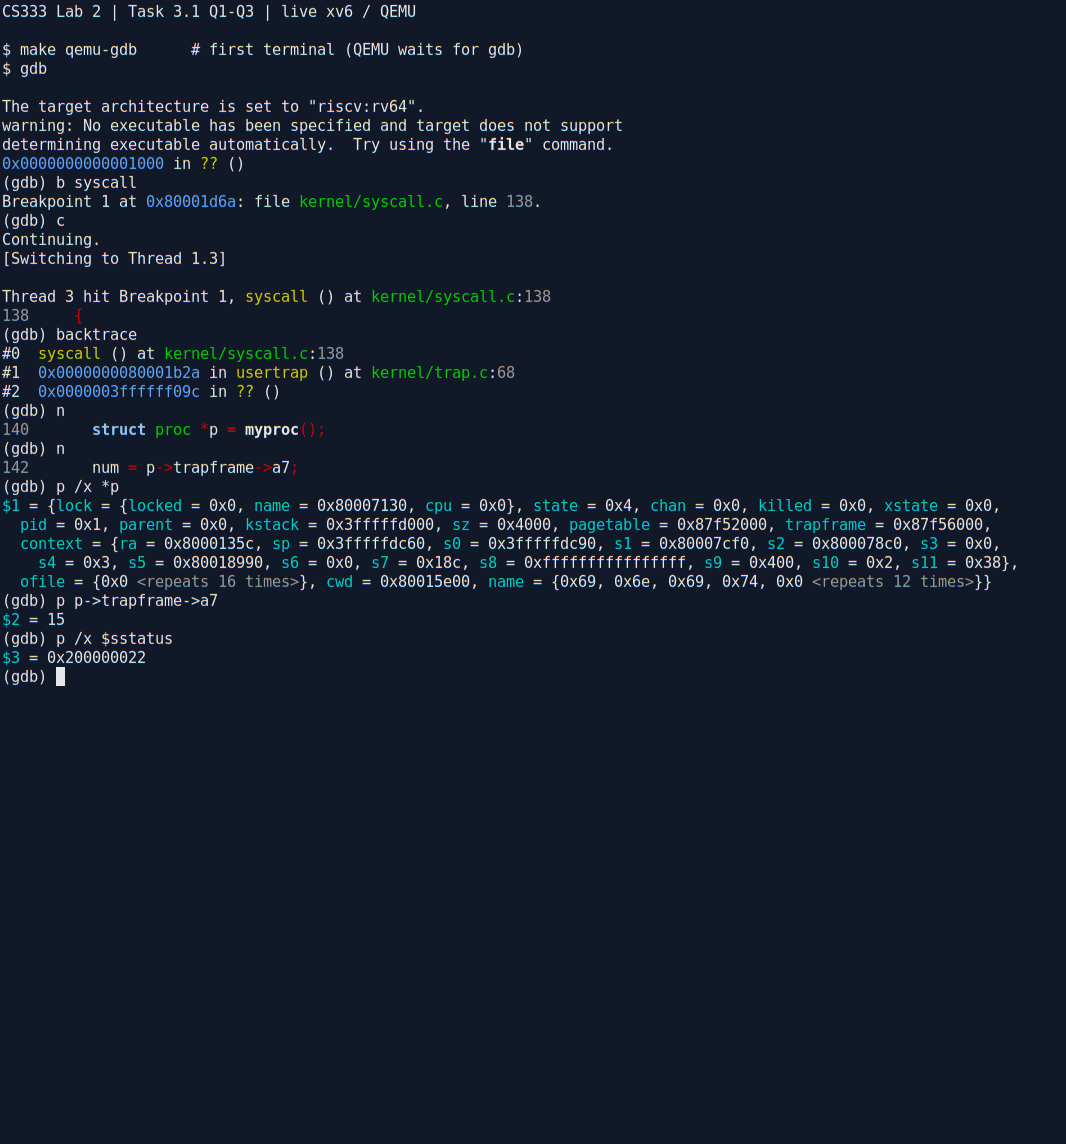
\includegraphics[width=0.82\linewidth,trim=0 456 46 170,clip]{gdb-syscall.png}
\caption{Breakpoint tại \cc{syscall}: \cc{backtrace}, nội dung \cc{struct proc}, \cc{trapframe->a7} và \cc{sstatus} (Q1–Q3).}\label{fig:gdb-syscall}
\end{figure}

\textbf{Q1. Hàm nào đã gọi \cc{syscall}?} Theo frame \cc{\#1} của \cc{backtrace}, đó là \cc{usertrap()} tại \cc{kernel/trap.c:68}. Frame \cc{\#2} ở địa chỉ \cc{0x3ffffff09c} = \cc{TRAMPOLINE + 0x9c}, chính là nhãn \cc{userret}: \cc{uservec} gọi \cc{usertrap()} bằng lệnh \cc{jalr t0}, nên địa chỉ trả về là lệnh ngay sau nó. GDB hiện \cc{??} vì mã trampoline được link ở \cc{0x80006000} (symbol \cc{uservec}), còn khi chạy nó được map ở địa chỉ ảo \cc{TRAMPOLINE = MAXVA - PGSIZE = 0x3ffffff000}.

\textbf{Q2. Giá trị của \cc{p->trapframe->a7} là gì và nó biểu diễn điều gì?} \cc{a7 = 15}, tức \cc{SYS\_open} trong \cc{kernel/syscall.h}. Stub trong \cc{user/usys.S} nạp số hiệu system call vào \cc{a7} rồi gọi \cc{ecall}; \cc{uservec} lưu các thanh ghi user vào trapframe, và \cc{syscall()} đọc lại \cc{a7} từ đó để chọn hàm xử lý.

Gợi ý của đề (xem \cc{user/initcode.S}, nơi giá trị là \cc{SYS\_exec}) dựa trên bản xv6 cũ. Bản 2026 không còn tệp này: \cc{forkret()} (\cc{kernel/proc.c}) gọi trực tiếp \cc{kexec("/init")} trong kernel cho process đầu tiên. Vì vậy system call đầu tiên đi qua \cc{syscall()} là \cc{open("console", O\_RDWR)} ở đầu \cc{main} của \cc{user/init.c}. Kết quả \cc{p /x *p} khẳng định điều này: \cc{pid = 0x1}, \cc{name = \{0x69, 0x6e, 0x69, 0x74\}} = \cc{"init"}, \cc{state = 0x4} (\cc{RUNNING}).

\textbf{Q3. CPU đang ở mode nào trước đó?} \textbf{User mode.} \cc{p /x \$sstatus} cho \cc{0x200000022}. Bit \cc{SPP} (bit 8) lưu mode trước khi trap: 0 là user, 1 là supervisor. Các bit khác cũng khớp với đường đi của system call (Hình~\ref{fig:sstatus}).

\begin{figure}[H]
\centering
\begin{tikzpicture}[x=0.4cm,y=1cm,font=\scriptsize]
  \newcommand{\fld}[5]{%
    \draw[hcmus,fill=#5] (#1,0) rectangle (#2,0.6);
    \node at ({(#1+#2)/2},0.3) {#4};
    \node[font=\tiny,text=gray] at ({(#1+#2)/2},0.8) {#3};}
  \fld{0}{3}{63–34}{0}{white}
  \fld{3}{6.6}{33–32}{\textbf{UXL = 10}}{boxbg}
  \fld{6.6}{9.6}{31–9}{0}{white}
  \fld{9.6}{12.6}{8}{\textbf{SPP = 0}}{hcmus!22}
  \fld{12.6}{14}{7–6}{0}{white}
  \fld{14}{17}{5}{\textbf{SPIE = 1}}{boxbg}
  \fld{17}{18.4}{4–2}{0}{white}
  \fld{18.4}{21.2}{1}{\textbf{SIE = 1}}{boxbg}
  \fld{21.2}{22.2}{0}{0}{white}
  \node[anchor=west,align=left,font=\scriptsize] at (23,0.3)
    {\cc{SPP = 0}: trap đến từ user mode\\
     \cc{SPIE = 1}: trước trap, ngắt đang bật\\
     \cc{SIE = 1}: \cc{usertrap()} gọi \cc{intr\_on()} trước \cc{syscall()}\\
     \cc{UXL = 2}: user mode dùng thanh ghi 64 bit};
\end{tikzpicture}
\caption{Giải mã \cc{sstatus = 0x200000022}.}\label{fig:sstatus}
\end{figure}

\textbf{Q4. Lệnh assembly nào gây panic? Thanh ghi nào ứng với biến \cc{num}?} Thay \cc{num = p->trapframe->a7;} bằng \cc{num = * (int *) 0;} rồi chạy \cc{make qemu}, kernel in \cc{scause=0xd sepc=0x80001d7a stval=0x0} và \cc{panic: kerneltrap}. Tìm \cc{80001d7a} trong \cc{kernel/kernel.asm} (Hình~\ref{fig:panic}, trái) được lệnh
\begin{center}\cc{80001d7a:\ \ 00002683\ \ \ \ lw\ \ a3,0(zero)}\end{center}
tức nạp 4 byte từ địa chỉ \cc{zero + 0} = \cc{0} vào thanh ghi \cc{a3}. Vậy \cc{num} nằm trong \textbf{\cc{a3}}; lệnh kế tiếp \cc{addiw a4,a3,-1} dùng \cc{a3} để kiểm tra \cc{num > 0 \&\& num < NELEM(syscalls)}. Trong gdb, breakpoint \cc{b *0x80001d7a} dừng đúng tại dòng 142 của \cc{syscall.c} và \cc{x/i \$pc} hiện cùng lệnh (Hình~\ref{fig:panic}, phải).

\begin{figure}[H]
\centering
\begin{minipage}[t]{0.555\linewidth}
\vspace{0pt}
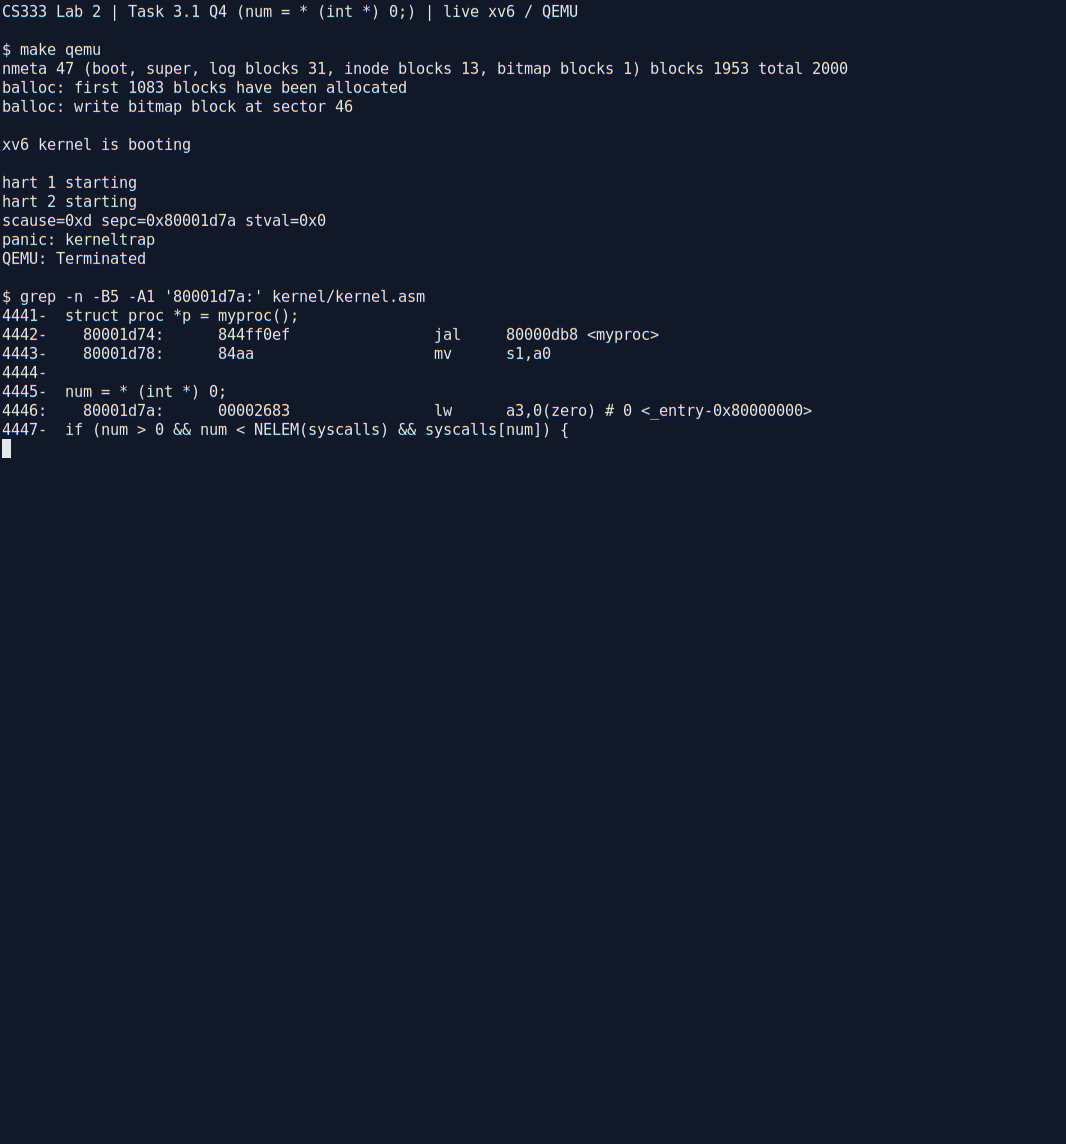
\includegraphics[width=\linewidth,trim=0 684 216 38,clip]{panic-asm.png}
\end{minipage}\hfill
\begin{minipage}[t]{0.425\linewidth}
\vspace{0pt}
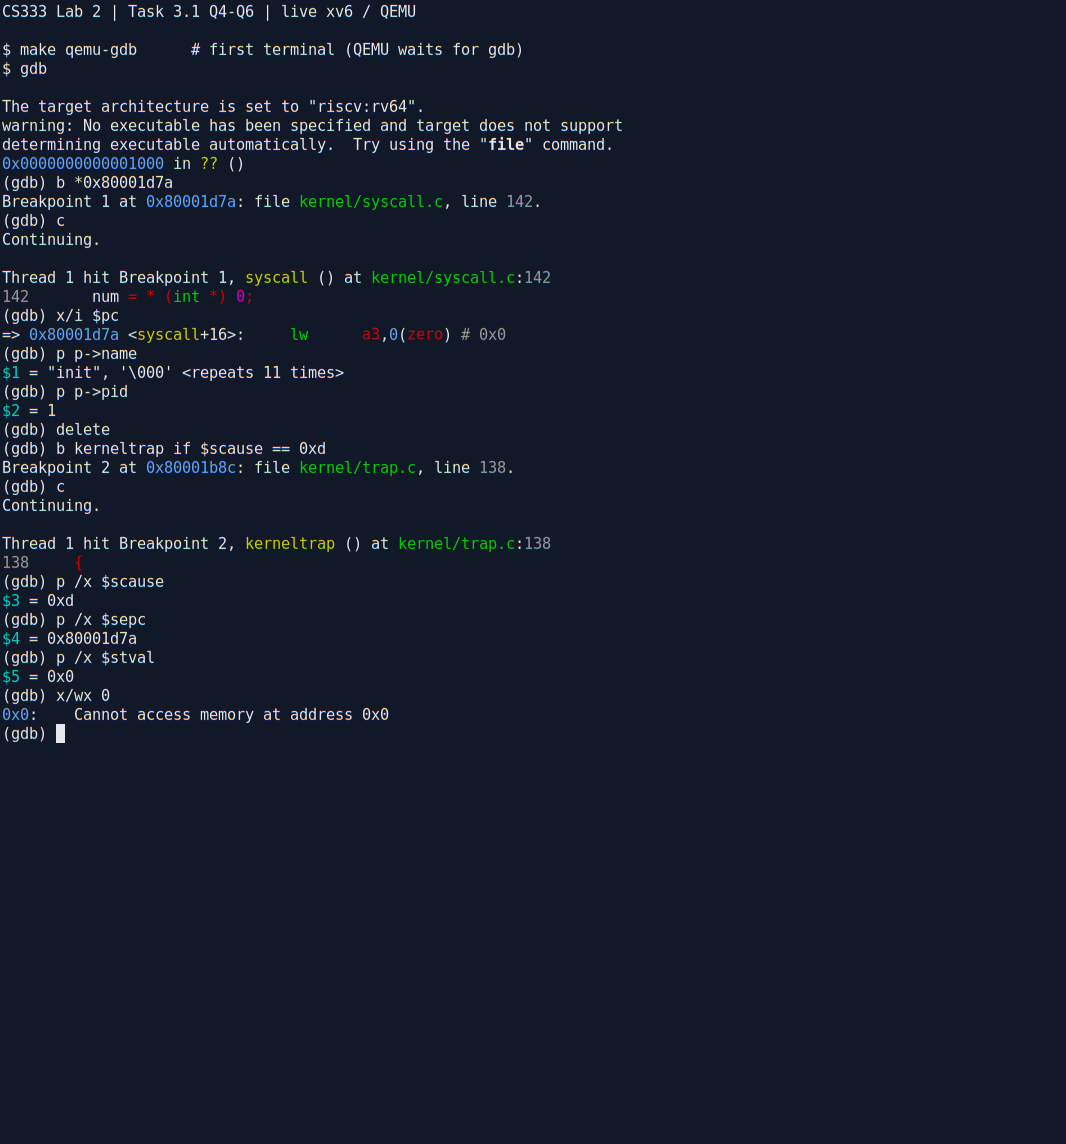
\includegraphics[width=\linewidth,trim=0 399 440 170,clip]{gdb-panic.png}
\end{minipage}
\caption{Trái: panic khi đọc địa chỉ 0 và lệnh tương ứng trong \cc{kernel.asm}. Phải: gdb tại lệnh lỗi và tại \cc{kerneltrap} (Q4–Q6).}\label{fig:panic}
\end{figure}

\textbf{Q5. Vì sao kernel bị crash?}\par
\begin{minipage}[t]{0.55\linewidth}
\vspace{0pt}
Kernel xv6 chạy với phân trang bật, dùng kernel page table do \cc{kvmmake()} (\cc{kernel/vm.c}) tạo. Bảng này chỉ map các vùng ở bảng bên, khớp Hình 3-3 của sách xv6; địa chỉ ảo \cc{0} không thuộc vùng nào. Khi lệnh \cc{lw} đọc địa chỉ 0, MMU không tìm được PTE hợp lệ và sinh exception:
\begin{itemize}
  \item \cc{scause = 0xd} = 13: \emph{load page fault} (bit ngắt = 0, mã exception 13 theo đặc tả RISC-V privileged);
  \item \cc{stval = 0x0}: địa chỉ ảo gây lỗi;
  \item \cc{sepc = 0x80001d7a}: lệnh \cc{lw} gây lỗi.
\end{itemize}
Trap đi vào \cc{kernelvec} rồi \cc{kerneltrap()}. Đây không phải ngắt thiết bị và kernel không bao giờ được phép page fault, nên \cc{kerneltrap()} in ba thanh ghi trên rồi gọi \cc{panic("kerneltrap")}. GDB xác nhận bằng breakpoint có điều kiện \cc{b kerneltrap if \$scause == 0xd}: \cc{\$scause = 0xd}, \cc{\$sepc = 0x80001d7a}, \cc{\$stval = 0x0}. Lệnh \cc{x/wx 0} cũng không đọc được địa chỉ 0.
\end{minipage}\hfill
\begin{minipage}[t]{0.42\linewidth}
\vspace{0pt}
\centering\small
\begin{tabularx}{\linewidth}{@{}X l c@{}}
\headrow \thd{Vùng} & \thd{Địa chỉ ảo} & \thd{Quyền} \\
PLIC & \cc{0x0c000000}–\cc{0x10000000} & RW \\
\rowcolor{rowalt}
UART0 & \cc{0x10000000} (1 trang) & RW \\
VIRTIO0 & \cc{0x10001000} (1 trang) & RW \\
\rowcolor{rowalt}
Mã kernel & \cc{0x80000000}–\cc{etext} & RX \\
Dữ liệu + RAM & \cc{etext}–\cc{0x88000000} & RW \\
\rowcolor{rowalt}
Kernel stack & dưới \cc{TRAMPOLINE} & RW \\
Trampoline & \cc{0x3ffffff000} & RX \\
\bottomrule
\end{tabularx}
\captionof{table}{Các vùng được map trong kernel page table; \cc{0x0} nằm ngoài tất cả.}
\vspace{4pt}
\begin{pseudobox}\small
Cùng địa chỉ 0 lại \emph{hợp lệ} trong user page table, vì mã của chương trình user bắt đầu ở địa chỉ ảo 0. Kernel page table không map bộ nhớ user, nên kernel phải đọc dữ liệu user qua \cc{copyin}/\cc{fetchaddr}.
\end{pseudobox}
\end{minipage}

\textbf{Q6. Process nào đang chạy khi kernel panic? PID là bao nhiêu?} Tại breakpoint \cc{0x80001d7a}: \cc{p p->name} = \cc{"init"}, \cc{p p->pid} = \cc{1}. Đó là process \textbf{\cc{init}} (PID 1), đang thực hiện system call đầu tiên, nên shell chưa kịp khởi động. Sau khi trả lời, câu lệnh \cc{num = p->trapframe->a7;} được khôi phục (script tự khôi phục và \cc{git status} sạch).

% =================================================================== 4
\section{Task 3.2 – Sandbox a command}

\textbf{Yêu cầu.} Thêm system call \cc{int interpose(int mask, const char *path)}. Nếu bit \cc{n} của \cc{mask} được bật thì system call số \cc{n} của process gọi \emph{không được thực thi} và trả về $-1$. Process con tạo bằng \cc{fork} thừa hưởng hạn chế của cha. Ở task này \cc{path} luôn là \cc{"-"} (được dùng ở Task 3.3).

\subsection{Các tệp đã sửa và trường mới trong \cc{struct proc}}
\begin{table}[H]
\centering\small
\begin{tabularx}{\linewidth}{@{}l X@{}}
\headrow \thd{Tệp} & \thd{Thay đổi} \\
\cc{Makefile} & Thêm \cc{\$U/\_sandbox}, \cc{\$U/\_sbtest} vào \cc{UPROGS} (khối \cc{ifeq (\$(LAB),syscall)}). \\
\rowcolor{rowalt}
\cc{kernel/syscall.h} & \cc{\#define SYS\_interpose 23}. \\
\cc{user/usys.pl}, \cc{user/user.h} & \cc{entry("interpose")} sinh stub trong \cc{user/usys.S}; khai báo \cc{int interpose(int, const char *)}. \\
\rowcolor{rowalt}
\cc{kernel/syscall.c} & Khai báo \cc{sys\_interpose}, thêm \cc{[SYS\_interpose]} vào bảng \cc{syscalls[]}; hàm \cc{sandbox\_rejects()} và phép kiểm tra trong \cc{syscall()}. \\
\cc{kernel/sysproc.c} & Hàm xử lý \cc{sys\_interpose()}. \\
\rowcolor{rowalt}
\cc{kernel/proc.h}, \cc{kernel/proc.c} & Trường \cc{sbmask}; \cc{kfork()} sao chép cho con; \cc{freeproc()} đặt lại 0. \\
\bottomrule
\end{tabularx}
\caption{Các tệp được sửa trong Task 3.2.}
\end{table}

\begin{table}[H]
\centering\small
\begin{tabularx}{\linewidth}{@{}l l X X@{}}
\headrow \thd{Trường} & \thd{Kiểu} & \thd{Ý nghĩa} & \thd{Vòng đời} \\
\cc{sbmask} & \cc{int} & Bit \cc{n} = 1 thì system call số \cc{n} bị từ chối. & Ghi bởi \cc{sys\_interpose()} (chỉ OR thêm bit); \cc{kfork()} sao chép; \cc{kexec()} giữ nguyên; \cc{freeproc()} đặt 0. \\
\rowcolor{rowalt}
\tbd & & Pathname được phép (Task 3.3). & \\
\bottomrule
\end{tabularx}
\caption{Các trường mới trong \cc{struct proc} (\cc{kernel/proc.h}).}
\end{table}

\subsection{Đường đi của lời gọi \cc{interpose} và của một system call bị chặn}
Hình~\ref{fig:interpose} theo dõi lệnh \cc{sandbox 32768 - cat README}. \cc{sandbox} fork một process con; process con gọi \cc{interpose(32768, "-")} rồi \cc{exec} chương trình \cc{cat}. $32768 = 2^{15}$ = \cc{1 << SYS\_open}.

\begin{figure}[H]
\centering
\begin{tikzpicture}[font=\scriptsize,
  box/.style={draw=hcmus,fill=white,rounded corners=2pt,align=center,inner sep=2.5pt,text width=2.55cm,minimum height=1.3cm},
  bad/.style={box,fill=todo!7,draw=todo},
  arr/.style={-{Stealth[length=2mm]},semithick,hcmus},
  lbl/.style={font=\scriptsize\itshape,text=hcmus,fill=white,inner sep=1pt}]
  \fill[hcmus!5] (-0.55,0.9) rectangle (16.5,-0.9);
  \fill[hcmus!12] (-0.55,-1.65) rectangle (16.5,-4.25);
  \node[rotate=90,font=\scriptsize\bfseries,text=hcmus] at (-0.3,0) {USER};
  \node[rotate=90,font=\scriptsize\bfseries,text=hcmus] at (-0.3,-2.95) {KERNEL};
  \node[box] (u1) at (1.35,0) {\textbf{sandbox} (con)\\\cc{interpose(32768,"-")}\\stub: \cc{a7} = 23; \cc{ecall}};
  \node[box] (k1) at (3.65,-2.65) {\textbf{syscall()}: \cc{num} = 23\\bit 23 = 0 $\rightarrow$\\\cc{sys\_interpose()}\\\cc{sbmask |= 0x8000}};
  \node[box] (u2) at (5.95,0) {\cc{interpose} trả 0\\\cc{exec("cat", argv)}\\(\cc{a7} = 7, bit 7 = 0)};
  \node[box] (k2) at (8.25,-2.65) {\textbf{kexec()}\\nạp ảnh của \cc{cat},\\giữ \cc{struct proc}:\\\cc{sbmask} = \cc{0x8000}};
  \node[box] (u3) at (10.55,0) {\textbf{cat}\\\cc{open("README")}\\stub: \cc{a7} = 15; \cc{ecall}};
  \node[bad] (k3) at (12.85,-2.65) {\textbf{syscall()}: \cc{num} = 15\\bit 15 = 1: \textbf{chặn}\\\cc{a0} = $-1$, \emph{không}\\gọi \cc{sys\_open()}};
  \node[box] (u4) at (15.15,0) {\cc{open} trả $-1$\\\cc{cat} in\\\cc{cannot open README}};
  \draw[arr] ($(u1.south)+(0.45,0)$) -- node[lbl]{ecall} ($(k1.north)+(-0.45,0)$);
  \draw[arr] ($(k1.north)+(0.45,0)$) -- node[lbl]{sret, \cc{a0}=0} ($(u2.south)+(-0.45,0)$);
  \draw[arr] ($(u2.south)+(0.45,0)$) -- node[lbl]{ecall} ($(k2.north)+(-0.45,0)$);
  \draw[arr] ($(k2.north)+(0.45,0)$) -- node[lbl]{sret} ($(u3.south)+(-0.45,0)$);
  \draw[arr] ($(u3.south)+(0.45,0)$) -- node[lbl]{ecall} ($(k3.north)+(-0.45,0)$);
  \draw[arr,todo] ($(k3.north)+(0.45,0)$) -- node[lbl,text=todo]{sret, \cc{a0}=$-1$} ($(u4.south)+(-0.45,0)$);
  \node[font=\scriptsize,text=hcmus,align=center] at (8,-3.95)
    {Mỗi lần \cc{ecall}: \cc{uservec} lưu thanh ghi user vào trapframe $\rightarrow$ \cc{usertrap()} (\cc{scause = 8}, \cc{epc += 4}) $\rightarrow$ \cc{syscall()} $\rightarrow$ kết quả vào \cc{trapframe->a0} $\rightarrow$ \cc{userret}, \cc{sret}};
\end{tikzpicture}
\caption{\cc{interpose} ghi mask vào \cc{struct proc}; mask sống qua \cc{exec} và chặn \cc{open} của \cc{cat} ngay tại dispatcher.}\label{fig:interpose}
\end{figure}

\subsection{Thiết kế và cài đặt}
\begin{itemize}
  \item \textbf{Kiểm tra một lần, trước khi gọi handler.} Phép kiểm tra nằm trong \cc{syscall()}, sau khi \cc{num} đã được xác nhận nằm trong bảng ($1 \le \cc{num} \le 23$, nên phép dịch \cc{sbmask >> num} luôn hợp lệ với \cc{int} 32 bit). System call bị chặn không chạy handler nên không có tác dụng phụ: \cc{fork} bị chặn không tạo process con. Cách này không phải sửa từng handler, và chặn được cả system call không có đối số như \cc{getpid}, \cc{fork} (test \cc{sandbox\_block}).
  \item \textbf{Hạn chế chỉ được cộng dồn.} \cc{sys\_interpose()} dùng \cc{|=} chứ không gán. Test \cc{sandbox\_escape} chạy \cc{sbtest escape} dưới mask \cc{open}; chương trình gọi \cc{interpose(0, 0)} và \cc{interpose(0, "README")} để thử thoát. Nếu dùng phép gán, mask 0 xóa luôn bit 15 và process tự thoát sandbox.
  \item \textbf{Kế thừa qua \cc{fork}, giữ qua \cc{exec}.} \cc{kfork()} sao chép \cc{sbmask} cho process con. \cc{kexec()} thay ảnh bộ nhớ nhưng giữ \cc{struct proc}, nên mask đặt trước \cc{exec} vẫn còn hiệu lực. Nhờ vậy \cc{sandbox 32768 - sh < exec.sh} chặn được cả \cc{ls} do \cc{sh} fork ra (test \cc{sandbox\_fork}).
  \item \textbf{Khởi tạo đúng cho process mới.} \cc{freeproc()} đặt \cc{sbmask = 0} cùng chỗ với \cc{pid}, \cc{killed}, \cc{xstate}. \cc{allocproc()} chỉ cấp slot \cc{UNUSED}, tức slot đã qua \cc{freeproc()} hoặc mảng \cc{proc[]} tĩnh vốn bằng 0, nên process không tạo bằng fork không thể nhận mask cũ.
  \item \textbf{Đồng bộ.} \cc{sbmask} chỉ được process tự đọc/ghi (trong \cc{syscall()}, \cc{sys\_interpose()}), được \cc{kfork()} ghi trước khi process con thành \cc{RUNNABLE}, và được \cc{freeproc()} ghi khi process đã kết thúc. Vì vậy trường này thuộc nhóm “private to the process” như \cc{sz}, \cc{pagetable}, không cần giữ \cc{p->lock}.
\end{itemize}

\srcname{kernel/syscall.c – kiểm tra sandbox tại dispatcher}
\begin{lstlisting}[firstnumber=138]
// Does the sandbox set up by interpose() reject system call num for p?
static int
sandbox_rejects(struct proc *p, int num)
{
  return (p->sbmask >> num) & 1;
}
\end{lstlisting}
\vspace{-2pt}
\begin{lstlisting}[firstnumber=151]
  num = p->trapframe->a7;
  if (num > 0 && num < NELEM(syscalls) && syscalls[num]) {
    if (sandbox_rejects(p, num)) {
      // Fail without running the handler.
      p->trapframe->a0 = -1;
    } else {
      // Use num to lookup the system call function for num, call it,
      // and store its return value in p->trapframe->a0
      p->trapframe->a0 = syscalls[num]();
    }
\end{lstlisting}

\begin{minipage}[t]{0.5\linewidth}
\vspace{0pt}
\srcname{kernel/sysproc.c – sys\_interpose}
\begin{lstlisting}[firstnumber=117,xleftmargin=22pt]
uint64
sys_interpose(void)
{
  int mask;

  argint(0, &mask);
  myproc()->sbmask |= mask;
  return 0;
}
\end{lstlisting}
\end{minipage}\hfill
\begin{minipage}[t]{0.47\linewidth}
\vspace{0pt}
\srcname{kernel/proc.c – kfork() và freeproc()}
\begin{lstlisting}[firstnumber=293,xleftmargin=22pt]
  // the child stays in the parent's sandbox.
  np->sbmask = p->sbmask;
\end{lstlisting}
\vspace{-2pt}
\begin{lstlisting}[firstnumber=170,xleftmargin=22pt]
  p->sbmask = 0;
\end{lstlisting}
\small \cc{argint(0, \&mask)} đọc đối số thứ nhất từ \cc{trapframe->a0}; mask mới được OR vào mask cũ. Đối số \cc{path} (\cc{a1}) chưa được đọc ở task này.
\end{minipage}

\subsection{Chạy thử}
\begin{minipage}[c]{0.27\linewidth}
\centering
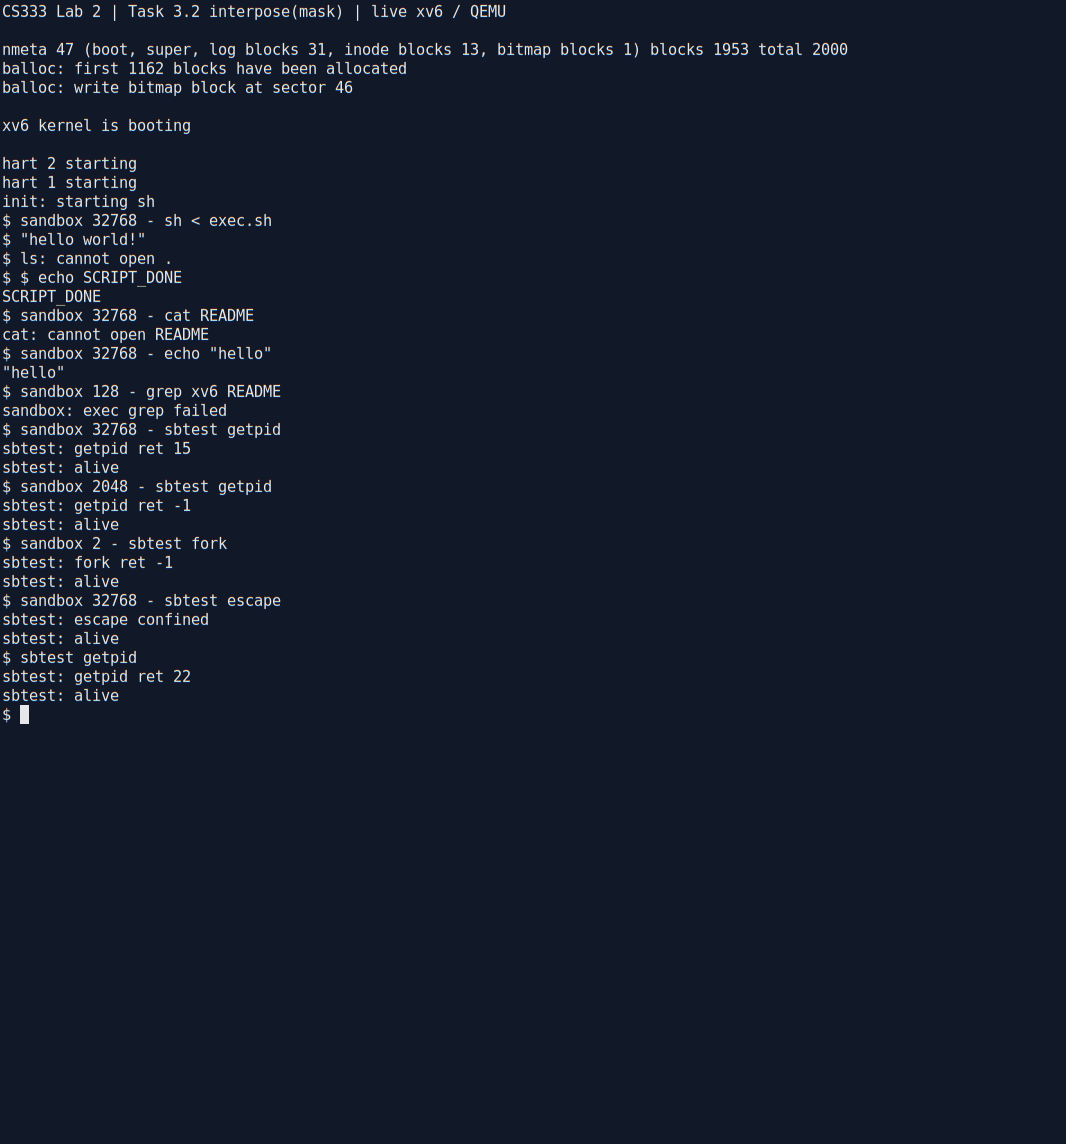
\includegraphics[width=\linewidth,trim=0 420 770 192,clip]{sandbox.png}
\captionof{figure}{Các mask khác nhau trong xv6.}\label{fig:sandbox}
\end{minipage}\hfill
\begin{minipage}[c]{0.7\linewidth}
\small
\begin{tabularx}{\linewidth}{@{}l l X@{}}
\headrow \thd{Mask} & \thd{Bit} & \thd{Kết quả} \\
32768 & \cc{open} (15) & \cc{sh < exec.sh}: \cc{echo} vẫn in \cc{"hello world!"}, \cc{ls} báo \cc{cannot open .}; \cc{cat}: \cc{cannot open README}; \cc{echo} không mở tệp nên chạy bình thường. \\
\rowcolor{rowalt}
128 & \cc{exec} (7) & \cc{sandbox: exec grep failed}: chính process con của \cc{sandbox} không exec được. \\
32768 & \cc{open} (15) & \cc{sbtest getpid} trả PID thật (15): system call không bị mask vẫn chạy. \\
\rowcolor{rowalt}
2048 & \cc{getpid} (11) & \cc{getpid ret -1}, process vẫn \cc{alive}. \\
2 & \cc{fork} (1) & \cc{fork ret -1}, không có dòng \cc{CHILD RAN}: handler không chạy. \\
\rowcolor{rowalt}
32768 & \cc{open} (15) & \cc{sbtest escape}: \cc{escape confined}. \\
-- & -- & \cc{sbtest getpid} chạy sau cùng, ngoài sandbox, trả PID 22: slot process tái sử dụng không giữ mask cũ. \\
\bottomrule
\end{tabularx}
\end{minipage}

% =================================================================== 5
\section{Task 3.3 – Sandbox with allowed pathnames}

\begin{todobox}
\textbf{CHỜ BỔ SUNG (Phạm Lê Huy Hoàng).} Theo mục 5.2 của đề: trường pathname mới trong \cc{struct proc} (bổ sung vào bảng trường ở mục 4.1), cách lấy \cc{path} bằng \cc{argstr} vào buffer \cc{MAXPATH}, xử lý \cc{"-"}, phép so sánh pathname của \cc{open}/\cc{exec} (gợi ý: mở rộng \cc{sandbox\_rejects()}), kế thừa qua \cc{fork}, danh sách tệp đã sửa và đường đi của một lời gọi \cc{open}/\cc{exec} được phép. Lưu ý \cc{sbtest escape} gọi lại \cc{interpose(0, "README")}, và địa chỉ 0 hợp lệ trong user space nên \cc{interpose(0, 0)} không làm \cc{argstr} thất bại.
\end{todobox}

% =================================================================== 6
\section{Task 3.4 – Attack xv6}

\begin{todobox}
\textbf{CHỜ BỔ SUNG (Phạm Lê Huy Hoàng).} Giải thích vì sao tấn công thành công: trang vật lý nào của \cc{secret} được \cc{kalloc()} cấp lại cho \cc{attack}, secret nằm ở offset nào và cách xác định offset đó (đề trừ điểm nếu chỉ thử sai mà không giải thích).
\end{todobox}

% =================================================================== 7
\needspace{16\baselineskip} % giữ tiêu đề cùng trang với bảng test
\section{Kiểm thử}

\begin{table}[H]
\centering\small
\begin{tabularx}{\linewidth}{@{}c >{\raggedright\arraybackslash}p{5.8cm} X r@{}}
\headrow \thd{Task} & \thd{Test của autograder} & \thd{Nội dung} & \thd{Kết quả} \\
3.1 & \cc{answers-syscall.txt} & Tệp trả lời tồn tại, đủ nội dung (chấm tay) & OK 5/5 \\
\rowcolor{rowalt}
3.2 & \cc{sandbox\_mask} & Mask \cc{open}, \cc{exec}, cả hai; \cc{exec} bị chặn & OK 5/5 \\
3.2 & \cc{sandbox\_fork} & Mask được \cc{sh} và các process con thừa hưởng & OK 5/5 \\
\rowcolor{rowalt}
3.2 & \cc{sandbox\_block} & \cc{getpid}, \cc{fork} bị chặn trả $-1$, không chạy handler & OK 5/5 \\
3.2 & \cc{sandbox\_escape} & Gọi lại \cc{interpose} không gỡ được hạn chế & OK 5/5 \\
\rowcolor{rowalt}
3.3 & \cc{sandbox\_\{path,most,minus,forkpath\}} & Pathname được phép cho \cc{open}/\cc{exec} & \tbd \\
3.4 & \cc{attack} & In ra secret của lần chạy \cc{secret} trước & \tbd \\
\rowcolor{rowalt}
-- & \cc{time} & \cc{time.txt} chứa một số nguyên & \tbd \\
\bottomrule
\end{tabularx}
\caption{Các test của \cc{grade-lab-syscall}. Kết quả hiện tại của Task 3.1, 3.2 lấy từ \cc{./grade-lab-syscall} trên nhánh \cc{syscall}.}\label{tab:grade}
\end{table}

Mã của Task 3.2 biên dịch với \cc{-Wall -Werror} không có cảnh báo; cảnh báo \cc{RWX} của linker thuộc kernel gốc. Ngoài autograder, ảnh chạy thử ở Hình~\ref{fig:sandbox} kiểm tra thêm hai điều autograder không đo: system call không bị mask vẫn hoạt động trong sandbox, và process mới không nhận mask cũ.

\begin{todobox}
\textbf{CHỜ BỔ SUNG.} Ảnh chụp toàn bộ output \cc{make grade} sau khi hoàn thành cả bốn task (đề yêu cầu trong bảng tự đánh giá).
\end{todobox}

% =================================================================== 8
\section{Thảo luận và tự đánh giá}\label{sec:discussion}

\subsection{Khó khăn và cách khắc phục}
\begin{table}[H]
\centering\small
\begin{tabularx}{\linewidth}{@{}>{\raggedright\arraybackslash}p{4.2cm} >{\raggedright\arraybackslash}X >{\raggedright\arraybackslash}X@{}}
\headrow \thd{Vấn đề} & \thd{Nguyên nhân} & \thd{Cách khắc phục} \\
Q2 gợi ý xem \cc{user/initcode.S} nhưng tệp không tồn tại & Bản xv6-labs-2026 chạy \cc{/init} trực tiếp bằng \cc{kexec()} trong \cc{forkret()} & Đọc \cc{forkret()} và \cc{user/init.c}; đối chiếu \cc{p->name = "init"}, \cc{pid = 1} để kết luận system call đầu tiên là \cc{open("console")}. \\
\rowcolor{rowalt}
\cc{si} tại lệnh \cc{lw} làm gdb báo \cc{target is running} và mất quyền điều khiển & Bước đơn đi vào trap trên QEMU nhiều hart & Đặt \cc{b kerneltrap if \$scause == 0xd} rồi \cc{c} để đọc \cc{scause}, \cc{sepc}, \cc{stval} ngay khi trap xảy ra. \\
\cc{sandbox 32768 - sh < exec.sh} chạy sau vài lệnh khác: process con của \cc{sh} bị page fault (\cc{scause 0xd}) trong \cc{malloc()} & Lỗi cố ý \cc{LAB\_SYSCALL}: \cc{uvmalloc()} không xóa trang, nên BSS của \cc{sh} vừa exec chứa rác, biến \cc{freep} (\cc{0x2010}) khác 0 & Tái hiện được cả khi \emph{không} dùng sandbox, nên đây không phải lỗi của Task 3.2. Autograder boot lại cho mỗi test; ảnh demo chạy lệnh này trước tiên. \\
\rowcolor{rowalt}
\tbd{} (Task 3.3, 3.4) & & \\
\bottomrule
\end{tabularx}
\caption{Các khó khăn gặp phải trong quá trình thực hiện.}
\end{table}

\subsection{Tự đánh giá theo thang điểm}
\begin{table}[H]
\centering\small
\begin{tabularx}{\linewidth}{@{}l c l X@{}}
\headrow \thd{Hạng mục} & \thd{Điểm tối đa} & \thd{Mức tự đánh giá} & \thd{Minh chứng} \\
1. Using gdb & 1.5 & Xuất sắc & 6/6 câu, mỗi câu có output gdb/ảnh chụp thật; \cc{answers-syscall.txt} đạt test. \\
\rowcolor{rowalt}
2a. \cc{interpose} plumbing & 0.5 & Xuất sắc & Đủ prototype, stub, số hiệu, bảng \cc{syscalls[]}, handler; build \cc{-Werror} không cảnh báo; \cc{sandbox}, \cc{sbtest} chạy. \\
2b. Mask rejection & 1.25 & Xuất sắc & \cc{sandbox\_mask}, \cc{sandbox\_block} đạt; kiểm tra một lần trong \cc{syscall()}; bị chặn thì trả $-1$, handler không chạy. \\
\rowcolor{rowalt}
2c. Inheritance by \cc{fork} & 0.75 & Xuất sắc & \cc{sandbox\_fork} đạt; \cc{kfork()} sao chép, \cc{freeproc()} đặt lại; demo không rò mask. \\
3a. Allowed pathname stored & 0.75 & \tbd & \\
\rowcolor{rowalt}
3b. \cc{open}/\cc{exec} path check & 1.75 & \tbd & \\
4. Attack xv6 & 2.0 & \tbd & \\
\rowcolor{rowalt}
5. Chất lượng mã, git, \cc{time.txt} & 0.5 & \tbd & Task 3.1–3.2: ba commit tách theo nội dung (trả lời gdb; plumbing; chặn và kế thừa mask). \\
6. Báo cáo & 1.0 & \tbd & \\
\bottomrule
\end{tabularx}
\caption{Tự đánh giá theo rubric của đề.}
\end{table}

% =================================================================== 9
\section{Tài liệu tham khảo}
\begin{enumerate}[label={[\arabic*]},leftmargin=2.2em,itemsep=3pt,before=\raggedright]
  \item CS333 – Hệ điều hành, \emph{Lab 2: System Calls} (đề bài, yêu cầu nộp bài và thang điểm), 2026.
  \item MIT 6.1810, \emph{Lab: System calls}, Fall 2026. \url{https://pdos.csail.mit.edu/6.828/2026/labs/syscall.html}
  \item R. Cox, M. F. Kaashoek, R. Morris, \emph{xv6: a simple, Unix-like teaching operating system (RISC-V)}, chương 2, chương 3 (Hình 3-3) và mục 4.3–4.4. \url{https://mit-pdos.github.io/xv6-riscv-book/}
  \item \emph{The RISC-V Instruction Set Manual, Volume II: Privileged Architecture} – thanh ghi \cc{sstatus}, mã \cc{scause}. \url{https://github.com/riscv/riscv-isa-manual}
  \item Mã nguồn xv6-labs-2026, nhánh \cc{syscall}: \cc{kernel/syscall.c}, \cc{kernel/trap.c}, \cc{kernel/trampoline.S}, \cc{kernel/proc.c}, \cc{kernel/vm.c}, \cc{kernel/kalloc.c}, \cc{kernel/memlayout.h}, \cc{user/init.c}, \cc{user/sandbox.c}, \cc{user/sbtest.c}.
  \item Công cụ AI (Claude Code): hỗ trợ tự động hóa và ghi lại phiên gdb, cài đặt và kiểm thử Task 3.2, soạn thảo báo cáo. Nhóm chịu trách nhiệm về toàn bộ nội dung bài nộp. \tbd{} (khai báo AI cho Task 3.3, 3.4 nếu có).
\end{enumerate}

\end{document}
